\documentclass[11pt,oneside,titlepage]{jsbook}

%%%--- Read Package ---%%%
\usepackage{times,array,fancyhdr,lastpage,amsmath,amssymb,txfonts,ccaption}
\usepackage{bm}
\usepackage[dvipdfm]{graphicx}
\usepackage[newitem,newenum]{paralist}%箇条書き書式変更スタイル
%\usepackage{slashbox}
\usepackage{bm}
\usepackage{here}
%\usepackage{subfigure}
\usepackage{comment}
\usepackage{type1cm}
\usepackage{amssymb}
\usepackage{cite}
\newcommand{\argmax}{\mathop{\rm max}\limits}

%%%--- Setup Layout ---%%%
\topmargin 0pt    %オフセットからヘッダまでのマージン
\headsep 35pt       %ヘッダと本文領域の間の高さ
\topskip 5pt        %本文領域内の本文開始位置までの高さ
\oddsidemargin 15pt %奇数ページのマージン
\footskip 30.00pt   %文章領域の終わりからフッタの終わりまでの高さ
\paperwidth 597pt   %用紙の幅
\paperheight 845pt  %用紙の高さ
\voffset 0pt        %垂直方向のオフセット
\hoffset 0pt        %水平方向のオフセット
\headheight 30pt    %ヘッダの高さ    
\evensidemargin 17pt%偶数ページのマージン
\marginparsep 10pt  %本文領域と傍注の間の幅
\marginparwidth 17pt%傍注の幅
\marginparpush 7pt  %傍注間の高さ
\textwidth 43zw     %文章領域の幅
\setlength{\textheight}{32.5\baselineskip}%行送り設定
\addtolength{\textheight}{\topskip}
\pagestyle{fancy}
\setcounter{tocdepth}{3}	%subsubsectionまでを目次に表示
\setcounter{secnumdepth}{4}

\begin{document}
\captiondelim{ }%キャプションの書式を変更
%↓fancy.styの設定
%\fancyhead{}
\rfoot{{\small 九州大学 大学院 システム情報科学府 情報知能工学専攻}}%右フッタ
%\fancyhead[LE]{\chaptermark}%偶数ページ左ヘッダ
%\fancyhead[LO]{\sectionmark}%奇数ページ左ヘッダ
\rhead{\textbf{\thepage}}   %右ヘッダ
\cfoot{}           %中央フッタ
\renewcommand{\headrulewidth}{0.4pt}
\renewcommand{\footrulewidth}{0.4pt}
\setlength{\baselineskip}{18.95pt}

%%%--- 章の最初のページのページ番号・ヘッダ・フッタを他のページと同じ形式で表示 ---%%% 
\makeatletter
\renewcommand{\chapter}{
  \if@openright\cleardoublepage\else\clearpage\fi
  \global\@topnum\z@
  \secdef\@chapter\@schapter}
\makeatother

%%%--- Title Page ---%%%
\vspace*{3cm}%\vspace*{長さ}:縦方向空白(ページ先頭有効)
\begin{center}%センタリングはじめ
{\Large \textbf{}}\\%\\:字下げ無し改行
\vspace{3mm}
{\Large \textbf{VectorCodingにおける伝搬路推定を必要としない\\固有符号推定アルゴリズム}} \\
\vspace{5cm}%\vspace{長さ}:縦方向空白(ページ先頭無効)
\indent \\
{\Large 仁部龍介} \\
\vspace{5mm}
{\Large 平成 31年 2月} \\
\vspace{5mm}
{\Large 修士課程 \\ 情報知能工学専攻 \\ 社会情報システム工学コース} \\
\end{center}%センタリングおわり 
\thispagestyle{empty}%\thispagestyle{ページスタイル名}:一時的にページスタイル変更
           %empty:ページ番号無し,plain:フッタ中央にページ番号を付ける

%\clearpage %\clearpage(改ページ)		

%\chapter*{概要} %章番号をつけない
\thispagestyle{empty}

\thispagestyle{empty}
近年,バックホール回線に無線回線を用いる無線中継網が進展している.一般的に,無線バックホール回線
における伝搬路は静的とされており,伝搬路情報の変動は比較的穏やかとされている.このような
条件下では,送受信機の両方にフィルタを置く通信方式を使用することができ,その一つとして
ベクトル符号化(VC:Vector Coding)が存在する.

ベクトル符号化は,伝搬路行列とその整合フィルタ(MF:Matched Filter)からなる合成チャネル行列の
固有ベクトルを拡散符号とするCDMである.合成チャネル行列のエルミート性から,固有ベクトルが
お互いに直交する点と,受信側におけるMFによってパスダイバーシチ効果を得る点を特徴とする.
固有ベクトルの獲得に関しては,これまでチャネル推定を用いた方法が数多く検討されてきた.
しかし,チャネル推定や推定した伝搬路情報から固有値分解によって固有ベクトルを得るには,
非常に多くの演算が必要となり,実装のハードルが高い.

そこで,本論文では膨大な演算を極めて簡単な非線形処理と無線機間反復処理で代替する手法,
Ping-Pong-Loop(PPL)を提案している.PPLは,べき乗法を基本原理とした,チャネル情報の
推定を必要としない固有ベクトル獲得を特徴とする.PPLは非常に少ない演算で固有ベクトルを
獲得できる点で,チャネル推定を用いる方法に対して優位性を持つが,固有ベクトルの獲得に
ある程度の無線機間反復数を要するという課題がある.また,ベクトル符号化自体にも,
小さい固有値に対応するチャネルにおいて,伝送するデータの誤り率が高くなるという課題がある.
本論文では,これらの課題に対して3つの検討を行った.無線機間反復数の削減に関しては,
伝送特性の劣悪なチャネルに対応する固有ベクトルを獲得せず,PPLを打ち切るアルゴリズムを
提案した.また,送信電力分配を適用することによって誤り率の高いチャネルの救済を行った.
そして,最後に送信電力分配を,固有ベクトル足切りアルゴリズムに適用し,これら3つに関して
シミュレーションを用いて検証を行った.


\frontmatter %ページ番号はローマ数字、章番号をつけない
\clearpage %\clearpage(改ページ)
%\pagenumbering{roman}
\tableofcontents %目次出力
\rhead{}

\mainmatter %ページ番号は算用数字、章番号をつける

\newpage
\rhead{\thepage}

\chapter{序論}
 
近年,スマートフォンやタブレット等の通信端末の急激な増加に伴い,大容量通信への期待が高まっている.
これを実現する有望な方策は小型の無線基地局を面的に多数設置し,面的周波数利用効率を高めること
である.しかしながら,無線基地局を多数設置するには基幹回線に接続するための有線バックホール回線を
要するため,その敷設コストの増大が問題となる.
そのため,バックホールとして無線中継網を用いる手法が検討されている~\cite{yamo} \cite{pabst}.
 ところで,一般的に,無線回線において高速伝送を行う場合,受信信号には遅延波による符号間干渉
 (信号歪み)が発生するため,適応等化等の信号歪みのへ対策技術が必須となる~\cite{akaiwa}.
 無線中継網の中継回線は端末の移動を伴うアクセス回線と比べて比較的静的であるため,
 その中継回線品質を高めるには送信機と受信機の双方で適応等化を行うことが有効である.

 線形フィルタを用いて送受信等化を実現する技術として,ベクトル符号化(\emph{VC:Vector Coding})~\cite{kasturia}が
知られている.ベクトル符号化は伝搬路相関行列の固有ベクトルを重み係数とする線形フィルタを
送受信で用いる方式であり,非線形の信号処理を行うことなく,信号電力対雑音電力比の最大化と
無歪み伝送(符号間干渉無し)を可能とする.また,無線LANや携帯電話システム等で広く採用されている
直交周波数分割多重(\emph{OFDM: Orthogonal Frequency Division Multiplexing})方式と異なり,
誤り訂正符号化を行うことなくパスダイバーシチ効果を得ることができるため~\cite{furukawa},
無線中継網等の固定回線通信においてはベクトル符号化がOFDMよりも優れた伝送特性を示すことが
期待できる~\cite{furukawa,li,takeda,takanashi}.しかしながら,ベクトル符号化を行うには送受信機双方でチャネル情報が必要となるため~\cite{furukawa},
チャネル推定とその固有値分解に非常に多くの演算が必要になる~\cite{takano} \cite{takeda2}.
これは,演算能力が限られた小型中継機を用いる場合,大きな制約となる.従来,べき乗法~\cite{strang}の原理に
基づき,固有値分解の演算を簡易な非線形処理と無線機間反復処理に置き換えるPing-Pong-Loop(PPL)が
提案されている.PPLは,任意ベクトルを2つの無線機間で反復処理することで,
徐々に合成チャネル行列の固有ベクトルに収束させる点を特徴とする.
しかしながら,PPLを用いることで送受信機の個々の演算量は軽減されるものの,
反復演算の収束値を得るために,特に固有値が小さい固有ベクトルを求めるために多大な無線機間反復を
こなす必要があり,解決すべき課題となる.
また,小さい固有値に対応する固有チャネルでは,チャネル利得が固有値の大きさに応じて小さくなることから,
比較的誤りやすくなるという課題がある.

本論文では,PPLにおける上記の課題を解決するために,以下の検討を行う.
第1に,獲得すべき固有ベクトル数を考慮したPPLにおける反復停止規範を提案する.
通信品質が基準以下である固有ベクトルに関してPPLの反復処理を停止することで,
獲得すべき固有ベクトルの足きりを行うものである.PPLアルゴリズムはべき乗法に基づくため,
固有値が小さい場合ほど収束が遅い. 提案方式では,固有値とBERの理論的な関係からPPLの反復毎に
BERを求め,それが所要値以下となる場合に演算を停止する.
それにより,不要な固有ベクトルを獲得する必要がないため,無線機間反復数を削減することができる.
第2に,PPLのための送信電力分配法を提案する.BER最少化規範に基づき送信電力を
各固有チャネルに最適分配することで利得の小さい固有チャネルの誤り率の改善を行う.
最後に,送信電力分配と足切りアルゴリズムを併用することで,反復回数を抑えながら,
一定の通信品質を満足するチャネル数の最大化を行う.

 本論文は以下のように構成される.第2章では提案手法の原理を支える数学的基礎概念と
ディジタル通信に関する基礎概念を説明する.第3章では提案アルゴリズムの根幹となるPPL過程について
説明を行い, 第4章にて本論文における検討方式の説明とシミュレーションによる検証を行う.
最後に第5章において,本論文のまとめと今後の展望について述べる.
 %序論
\chapter{基本的概念の解説}
本章では,本論文を理解する上で必要となる基本概念についての説明を行う.VCを理解するため材料として
エルミート行列の性質やべき乗法について説明する. \cite{strang} また,無線通信の理解に関してディジタル変復調,
同期検波等について説明を行う.

\section{数学的基礎知識}
VCを理解するための事前準備として数学的基礎知識の説明を行う.本章では行列の要素が複素数である
複素行列を扱っている.

\subsection{随伴行列(共役転置行列)}
ある複素行列$\bm{A}$において,全要素で共役をとった上でその行列を転置させたものを$\bm{A}$の随伴行列(共役転置行列)
といい,$\bm{A^H}$と表す.

(例)\quad
$
  \bm{A} = \left[
    \begin{array}{cc}
      1-i & 2-6i \\
      5+i & 3 \\
      0 & 1+9i
    \end{array}
  \right]
$とすると,
\vspace{1mm}
\begin{equation}
    \bm{A^H} = \left[
        \begin{array}{cc}
            1-i & 2-6i \\
            5+i & 3 \\
            0 & 1+9i
        \end{array}
    \right]^H 
    = \left[
        \begin{array}{ccc}
            1+i & 5-i & 0 \\
            2+6i & 3 & 1-9i \\
        \end{array}
    \right] \nonumber
\end{equation}

\subsection{複素ベクトルの内積}
要素数の等しい複素ベクトル$X,Y$の内積を,以下で定義する.
\begin{equation}
    (\bm{X},\bm{Y}) = \bm{X^HY}
\end{equation}

\subsection{任意ベクトルの表記}
M次元空間内の任意の列ベクトルを$\bm{x}$,M個の直交した固有ベクトルを$\bm{u_1},\bm{u_2},\ldots,\bm{u_M}$
とすると,$\bm{x}$はM個の固有ベクトル及び定数$c_i(i=0,1,\ldots,M)$を用いて,以下のように表すこと
ができる.
\begin{equation}
    \bm{x} = \sum_{i=1}^M c_i\bm{u_i}
\end{equation}

\section{エルミート行列}
ある複素行列$\bm{A}$において,$\bm{A}$の随伴行列$\bm{A^H}$が$\bm{A}$と等しいとき,$\bm{A}$を
エルミート行列と呼ぶ.

(例) \quad
$
  \bm{A} = \left[
    \begin{array}{cc}
      1 & 3-4i \\
      3+4i & 2
    \end{array}
  \right]
$とすると,
\vspace{1mm}
\begin{equation}
    \bm{A^H} = \left[
        \begin{array}{cc}
            1 & 3-4i \\
            3+4i & 2
        \end{array}
    \right]
    = \bm{A} \nonumber
\end{equation}
であり,$\bm{A^H}=\bm{A}$となることから$\bm{A}$はエルミート行列であると言える.

エルミート行列の主な性質として以下の4つが挙げられる.

\vspace{5mm}
\noindent\textbf{(性質1) \quad 任意複素ベクトルとの関係} \\
$\bm{A}$がエルミート行列であれば,任意の列ベクトル$\bm{x}$に対して,$\bm{x^HAx}$は実数になる.\\
\begin{comment}
\vspace{3mm}
(証明)

任意複素ベクトル
$
    \bm{x} = \left[
        \begin{array}{c}
            u \\
            v
        \end{array}
    \right]
$
,エルミート行列
$
    \bm{A} = \left[
        \begin{array}{cc}
            a & b \\
            b^* & c
        \end{array}
    \right]
$
とすると,
\begin{eqnarray}
    \bm{x^HAx} &=& 
    \left[
        \begin{array}{cc}
            u^* & v^*
        \end{array}
    \right]
    \left[
        \begin{array}{cc}
            a & b \\
            b^* & c
        \end{array}
    \right]
    \left[
        \begin{array}{c}
            u \\
            v
        \end{array}
    \right] \nonumber \\
    &=& auu^* + cvv^* + b^*uv^* + bu^*v \nonumber \\
    &=& a|u|^2+c|v|^2+b^*uv^*+bu^*v
\end{eqnarray}

\noindent(2.3)式の右辺第1項,第2項はともに実数である.第3項,第4項は互いに複素共役となっており,これらの
和は実数部分の2倍になる.よって,$\bm{x^HAx}$は実数であると言える.
\end{comment}

\vspace{5mm}
\noindent\textbf{(性質2) \quad 全固有値が実数} \\
エルミート行列の固有値はすべて実数である. \\

\begin{comment}
\vspace{3mm}
(証明) \\
エルミート行列$\bm{A}$の固有値を$\bm{\lambda}$,その$\bm{\lambda}$に対応する$\bm{0}$でない
固有ベクトルを$\bm{x}$とする.行列とその行列の固有値・固有ベクトルとの関係より,
\begin{equation}
    \bm{Ax} = \lambda\bm{x}
\end{equation}
(2.4)式の両辺に$\bm{x^H}$をかけると,
\begin{equation}
    \bm{x^HAx} = \lambda\bm{x^Hx}
\end{equation}
(2.5)式の左辺は(性質1)により実数である.加えて,$\bm{x}\neq\bm{0}$より,$\bm{x^Hx}=||x||^2$
は正の実数である.したがって,$\lambda$は実数でなければならない.
\end{comment}

\vspace{5mm}
\noindent\textbf{(性質3) \quad 固有ベクトルの直交性} \\
エルミート行列の固有ベクトルは,他のあらゆる固有値の固有ベクトルと直交している. \\

\begin{comment}
\vspace{3mm}
(証明) \\
ある$2\times2$以上の大きさを持ったエルミート行列$\bm{A}$の2つの異なる$\bm{0}$でない固有ベクトルを
$\bm{x}$,$\bm{y}$とし,$\bm{x}$,$\bm{y}$に対応する固有値を$\lambda,\mu(\lambda\neq\mu)$と
する.行列とその行列の固有値・固有ベクトルとの関係((2.4)式)より,
\begin{eqnarray}
    \bm{Ax} &=& \lambda\bm{x} \\
    \bm{Ay} &=& \mu\bm{y}
\end{eqnarray}
(2.6)式を共役転置すると,
\begin{equation}
    \bm{x^HA^H} = \lambda\bm{x^H} \hspace{10mm} (\because\lambda は実数より,\lambda=\lambda^*)
\end{equation}
$\bm{A}$はエルミート行列であることから$\bm{A=A^H}$.これを(2.8)式に代入して,
\begin{equation}
    \bm{x^HA} = \lambda\bm{x^H}
\end{equation}
(2.9)式の両辺に右から$\bm{y}$をかけると,
\begin{equation}
    \bm{x^HAy} = \lambda\bm{x^Hy}
\end{equation}
一方,(2.7)式の両辺に左から$\bm{x^H}$をかけると,
\begin{equation}
    \bm{x^HAy} = \mu\bm{x^Hy}
\end{equation}
これら(2.10)式,(2.11)式より,
\begin{equation}
    \lambda\bm{x^Hy} = \mu\bm{x^Hy}
\end{equation}
$\lambda\neq\mu$であることから,$\bm{x^Hy}=\bm{0}$でなければならない.$\bm{x^Hy}$は
複素列ベクトル$\bm{x},\bm{y}$の内積を表しており((2.1)式),それが$\bm{0}$であるということは
$\bm{x}$と$\bm{y}$は直交関係にある.
\end{comment}

\vspace{5mm}
\noindent\textbf{(性質4) \quad スペクトル定理} \\
エルミート行列$\bm{A}$はその固有ベクトル群行列$\bm{U}$,固有値対角行列$\bm{D}$を用いて,
次のように分解できる. \\
\begin{eqnarray}
    \bm{A} &=& \bm{UDU^H} = \lambda_1\bm{u_1u_1^H}+\lambda_2\bm{u_2u_2^H}+\ldots+\lambda_n\bm{u_nu_n^H} \nonumber \\
    &=& \sum_i \lambda_i\bm{u_iu_i^H}
\end{eqnarray}

\begin{comment}
\vspace{3mm}
(証明) \\
あるエルミート行列$\bm{A}$の固有値・固有ベクトルをそれぞれ$\lambda_i,\bm{u_i}$とする.
$\bm{u_i}$は正規直交基底であるから,任意ベクトル$\bm{x}$は(2.2)式のように分解される.
$\bm{x}$に左から$\bm{A}$をかけると,
\begin{equation}
    \bm{Ax} = \sum_i c_i\bm{Au_i} = \sum_i c_i\bm{\lambda u_i}
\end{equation}
が得られる.一方,(2.13)式の右辺に$\bm{x}$をかけると,
\begin{equation}
    \left[
        \sum_k \lambda_k\bm{u_ku_k^H}
    \right]\bm{x}
    = \left[
        \sum_k \lambda_k\bm{u_ku_k^H}
    \right]\sum_i c_i\bm{u_i}
    = \sum_{i,k} c_i\lambda_k\bm{u_ku_k^Hu_i}
    = \sum_i c_i\lambda_i\bm{u_i} \nonumber
\end{equation}
となり,これは(2.14)式と一致する.以上より,(2.13)式が成立することが証明された.
\end{comment}

\section{べき乗法}
対角行列の固有値・固有ベクトルを求める方法の一つにべき乗法がある.$\bm{A}$をM次のエルミート行列
とし,その固有値を$\lambda_1,\lambda_2,\ldots,\lambda_M$とする.$\lambda_i$に対応する
固有ベクトルを$\bm{u_i}$とすると,(2.4)式より,
\begin{equation}
    \bm{Au_i} = \lambda_i\bm{u_i} \nonumber
\end{equation}
となる.以下では,$|\lambda_1|>|\lambda_2|>\cdots>|\lambda_M|$の関係があるとする.
任意ベクトル$\bm{x}$に左から$\bm{A}$をn回乗算したものを$\bm{x_n}$とする.$\bm{x}$に左から
$\bm{A}$を1回乗算すると,
\begin{eqnarray}
    \bm{x_1} &=& \bm{Ax_0} = \bm{A}\sum_{i=1}^M c_i\bm{u_i} \hspace{10mm}(\because(2.2)式) \nonumber \\
    &=& \sum_{i=1}^M c_i\bm{Au_i} = \sum_{i=1}^M c_i\lambda_i\bm{u_i}
\end{eqnarray}
である.(2.15)式に繰り返し左から$\bm{A}$を1回乗算すると,
\begin{eqnarray}
    \bm{x_2} &=& \bm{Ax_1} = \bm{A^2x_0} = \sum_{i=1}^M c_i\lambda_i^2\bm{u_i} \nonumber \\
    \bm{x_3} &=& \bm{Ax_2} = \bm{A^3x_0} = \sum_{i=1}^M c_i\lambda_i^3\bm{u_i} \nonumber \\
    \vdots \nonumber
\end{eqnarray}
となり,$\bm{x_n}$は下記のようになる.
\begin{eqnarray}
    \bm{x_n} &=& \sum_{i=1}^M c_i\lambda_i^n\bm{u_i} \nonumber \\
    &=& \lambda_1^n
    \left(
        c_1+\bm{u_1}+\sum_{i=2}^M c_i
        \left(
            \frac{\lambda_i}{\lambda_1}
        \right)^n
        \bm{u_i}
    \right)
\end{eqnarray}
(2.16)式において,nが十分に大きい($\bm{A}$の乗算を十分繰り返す)場合,
\begin{equation}
    \left|\frac{\lambda_i}{\lambda_1}^n\right| << 1 \hspace{10mm} (i=2,3,\ldots,M)
\end{equation}
であるから,(2.16)式,(2.17)式より,
\begin{equation}
    \bm{x_n} = \lambda_1^nc_1\bm{u_1}
\end{equation}
が導かれる.(2.18)式は,任意ベクトル$\bm{x}$に繰り返し$\bm{A}$を乗算することで$\bm{x}$が
$\bm{A}$の第1(最大)固有ベクトル$\bm{u_1}$の定数倍に近づいていくことを意味している.
$\bm{x_n}$と$\bm{u_1}$は,大きさは違うが方向は同じであるため,$\bm{x_n}$を正規化することで
$\bm{u_1}$が得られる.正規化とはベクトルの各成分をベクトルの長さ(ノルム)で割ることにより,
ベクトルを単位ベクトルにすることである.

nを十分大きく取り$\bm{u_1}$を引き込んだ後,$\bm{u_1}$に$\bm{A}$を乗算することで$\bm{u_1}$に
対応する固有値$\lambda_1$は得られる.つまり,$\bm{u_1}$に$\bm{A}$を乗算した結果を$\bm{u_1^{\prime}}$
とすると,$\bm{u_1^{\prime}}$は$\bm{u_1}$の定数倍となり,この定数が固有値$\lambda_1$である.

エルミート行列$\bm{A}$はスペクトル定理により,(2.13)式のように分解できる.(2.13)式と一致する.以上より,
\begin{equation}
    \bm{A} - \lambda_1\bm{u_1}\bm{u_1^H} = \lambda_2\bm{u_2}\bm{u_2^H} + \cdots + \lambda_n\bm{u_n}\bm{u_n^H}
\end{equation}
であるから,(2.19)式の左辺$\bm{A} - \lambda_1\bm{u_1}\bm{u_1^H}$($\bm{A_2}$とする)の
第1固有値・固有ベクトルは,$\bm{A}$の第2固有値・固有ベクトルに当たる.すなわち,$\bm{A}$から
第1固有値・固有ベクトルを導出した手順を$\bm{A_2}$に適用することで,$\bm{A}$の第2固有値・
固有ベクトルが得られる.第2以降の固有値・固有ベクトルも,第2固有値・固有ベクトルと同様の手順で得られる.

\section{最適化問題の解法}
最適化問題は,与えられた制約条件の下で,目的関数と呼ばれる望ましさの尺度を表す関数が最小または最大となるような
決定変数の値を見つける,という数学モデルとして定式化できる. \cite{ibaragi}
最適化問題は,まず目的関数が線形関数か非線形関数かで大きく二つに分けることができる.そこからさらに,
制約条件の等号,不等号や決定変数が連続か非連続かによって細分化される.
一般に非線形関数の最適化の方が線形関数の最適化よりも困難とされる.

\subsection{KKT条件(Karush-Kuhn-Tucker condition)}
次のような不等式制約を持つ最適化問題を考える.

\begin{equation}
    \left\{
        \begin{array}{cc}
            目的関数:f(x) \to 最小 & \\
            制約条件:c_i(x) \leq 0 & (i=1,2,\ldots,m)
        \end{array}
    \right.
\end{equation}

ただし,変数$x$はn次元実ベクトルであり,目的関数$f:R^n \to R$および制約関数
$c_i:R^n \to R(i=1,\ldots,m)$はともに2回連続微分可能と仮定する.
まず,点$x$を(2.20)の実行可能解としたとき,$c_i(x)=0$が成り立つ制約条件を点$x$における有効制約
とよび,その集合を

\begin{equation}
    I(x) = {i| \quad c_i(x)=0 \hspace{10mm} (i=1,2,\ldots,m)} \nonumber
\end{equation}

で表す.さらに,有効制約の勾配ベクトル$\nabla c_i(x)(i \in I(x))$が1次独立であるような点$x$を
正則点という.

次の定理に示される条件は,非線形最適化問題の最適解を特徴づける重要な条件であり,KKT
(\emph{KKT: Karush Kuhn Tucker})条件と呼ばれる.\cite{ibaragi}

点$x^*$が(2.20)の局所的最適解かつ正則点ならば,

\begin{equation}
    \left\{
        \begin{array}{cccc}
            \nabla f(x^*)+\sum_{i=1}^m u_i^*\nabla c_i(x^*)=0 & & & \\
            c_i(x^*)\leq0, & u_i^*\geq0, & u_i^*c_i(x^*)=0 & (i=1,2,\ldots,m)
        \end{array}
    \right.
\end{equation}
を満たすベクトル$u^*=(u_1^*,u_2^*,\ldots,u_m^*)$が存在する.
ベクトル$u^*$をラグランジュ乗数と呼ぶ.

\subsection{ラグランジュの未定乗数法}
変数$\bm{x}$の関数$f(\bm{x})$の最大値,最小値は,等式制約$g(\bm{x})=0$が存在する場合,
ラグランジュ乗数$\lambda$を導入した

\begin{equation}
    F = f(\bm{x}) - \lambda g(\bm{x})
\end{equation}

を考え,これを$\bm{x}$で微分して$\bm{0}$と置く.

\begin{equation}
    \nabla_{\bm{x}}f - \lambda\nabla_{\bm{x}}g = \bm{0}
\end{equation}

これと等式制約$g(\bm{x})=0$を連立させて解けば,$\bm{x}$と$\lambda$を定めることができる.
この解法をラグランジュの未定乗数法と呼ぶ. \cite{kanatani}
ラグランジュの未定乗数法は線形最適化問題の解法として一般的である.
また,制約条件に不等式制約が存在する場合を考えるとき,ラグランジュの未定乗数法を
拡張した,2次計画法と呼ばれる解法が用いられる.
2次計画法を用いることでKKT条件の最適化問題を解くことができる.

\section{ディジタル変復調}
無線通信では,情報源のベースバンド信号(変調信号)を搬送波を用い,搬送波周波数帯の
信号に変換することが必要である.ベースバンド信号を伝送に適した形に変換することを変調と
呼び,逆の操作を復調と呼ぶ.これらの処理を合わせて変復調と呼び,その中でも情報源がディ
ジタルデータのものをディジタル変復調と呼ぶ\cite{takahata}.変調では,搬送波の振幅や周波数,位相な
どの性質を変化させることにより,信号を変換する.

\subsection{ディジタル変調}
\subsubsection{QPSK(Quadrature Phase Shift Keying)}
位相を用いて変調するものを位相偏移変調(PSK:Phase Shift Keying)と呼ぶ.
PSKでは,2進ディジタル信号を$n$ビットずつまとめ,これに対し$M=2^n$の位相を割り当てることで
搬送波に情報を持たせる.これを一般に$M$相PSKと呼び,
次の式で表される\cite{saitou}\cite{okumura}.
\begin{eqnarray}
\left\{
\begin{array}{ll}
\displaystyle s(t)=\mbox{Re}\left[Ae^{j(\omega_c t+\phi_m)}\right]&(-T/2 \leq t \leq T/2) \\[2mm]
\displaystyle \phi_m = \frac{2\pi}{M}(m-1) & (m=1,2, \cdots ,M)
\end{array}
\right.
\label{no2-6}
\end{eqnarray}
$M$相PSKの中でも$M$=4の場合を4位相偏移変調(QPSK:Quadrature Phase Shift Keying)と呼び,
$\phi_m=\pi/4,  3\pi/4,  5\pi/4,  7\pi/4$ が用いられる \cite{okumura}.
QPSK信号$S_{{\rm QPSK}}(t)$は,
\begin{eqnarray}
S_{{\rm QPSK}}(t)&=&\mbox{Re}\left[Ae^{j(\omega_c t +\phi_m)} \right] \nonumber \\
&=&\mbox{Re}\left[\left\{A\cos\phi_m+jA\sin\phi_m\right\}e^{j\omega_c t}\right] \nonumber \\[1mm]
&=&\mbox{Re}\left[\left\{Ad_1(t)+jAd_2(t) \right\}e^{j\omega_c t}\right] \nonumber \\[1mm]
&=&Ad_1(t)\cos\omega_ct-Ad_2(t)\sin\omega_ct
\label{eqqpsk}
\end{eqnarray}
と表される.ここで,
\begin{eqnarray}
\left\{
\begin{array}{ll}
\displaystyle \phi_m = \frac{2\pi}{4}(m-1)+\frac{\pi}{4} \hspace{2mm}(m=1,\cdots ,4) \\[2mm]
\displaystyle d_1 = \cos \phi_m \hspace{16mm}(=\pm1) \\[1mm]
\displaystyle d_2 = \sin \phi_m \hspace{16.5mm}(=\pm1)
\end{array}
\right.
\label{ff}
\end{eqnarray}
である.つまり,QPSKではこの4つの位相を2ビットの系列00,01,10,11に対応させて伝送する.
QPSK変調の信号点配置および,変調器の回路図を図\ref{fig:qpskIQ},図\ref{fig:qpskmod}に示す.
信号点配置はグレイコードが用いられ,隣接する信号点のハミング距離が1となるように設定されている.
%----------------------------画像をいれた----------------------------
\begin{figure}[t]
  \begin{center}
    \includegraphics[scale = 0.25]{./chapter2/figure/qpskiq.eps}
    \caption{QPSK変調の信号点配置の例}
    \label{fig:qpskIQ}
  \end{center}
\end{figure}
\begin{figure}[t]
  \begin{center}
    \includegraphics[scale = 0.25]{./chapter2/figure/qpskshift.eps}
    \caption{QPSK変調の回路図}
    \label{fig:qpskmod}
  \end{center}
\end{figure}

\subsection{同期検波}
変調された信号(被変調信号)から元の信号を得ることを復調という.復調方式として図 \ref{fig:qpskcoh} に示すような同期検波を考える.同期検波とは,変調側と同位相の搬送波を用い,受信信号との積をとることにより,元の変調信号を得る方法である\cite{takahata}.QPSK信号$S_{{\rm QPSK}}(t)$に$\cos\omega_c t$,$-\sin\omega_c t$をかけたものをそれぞれ$m_1(t), m_2(t)$とすると,
\begin{eqnarray}
m_1(t)&=&Ad_1(t)\cos^2\omega_ct+Ad_2(t)\sin\omega_ct\cos\omega_ct \nonumber \\
&=&\frac{1}{2}Ad_1(t)+\frac{1}{2}Ad_1(t)\cos2\omega_ct+\frac{1}{2}Ad_2(t)\sin2\omega_ct \\
m_2(t)&=&-Ad_1(t)\sin\omega_ct\cos\omega_ct+Ad_2(t)\sin^2\omega_ct \nonumber \\
&=&\frac{1}{2}Ad_2(t)-\frac{1}{2}Ad_2(t)\cos2\omega_ct-\frac{1}{2}Ad_1(t)\sin2\omega_ct
\end{eqnarray}
となる.ここで,$m_1(t)$,$m_2(t)$をローパスフィルタ(LPF:Low-Pass Filter)に通すことにより高周波成分を除いたものを$\hat{m}_1(t)$,$\hat{m}_2(t)$とすると,
\begin{eqnarray}
\hat{m}_1(t)&=&\frac{1}{2}Ad_1(t)\\
\hat{m}_2(t)&=&\frac{1}{2}Ad_2(t)
\end{eqnarray}
となる.$\hat{m}_1(t)$,$\hat{m}_2(t)$を並直列変換(parallel / serial conversion)することで,元の信号が復元される.
%------------------------------仮画像------------------------------
\begin{figure}[t]
  \begin{center}
    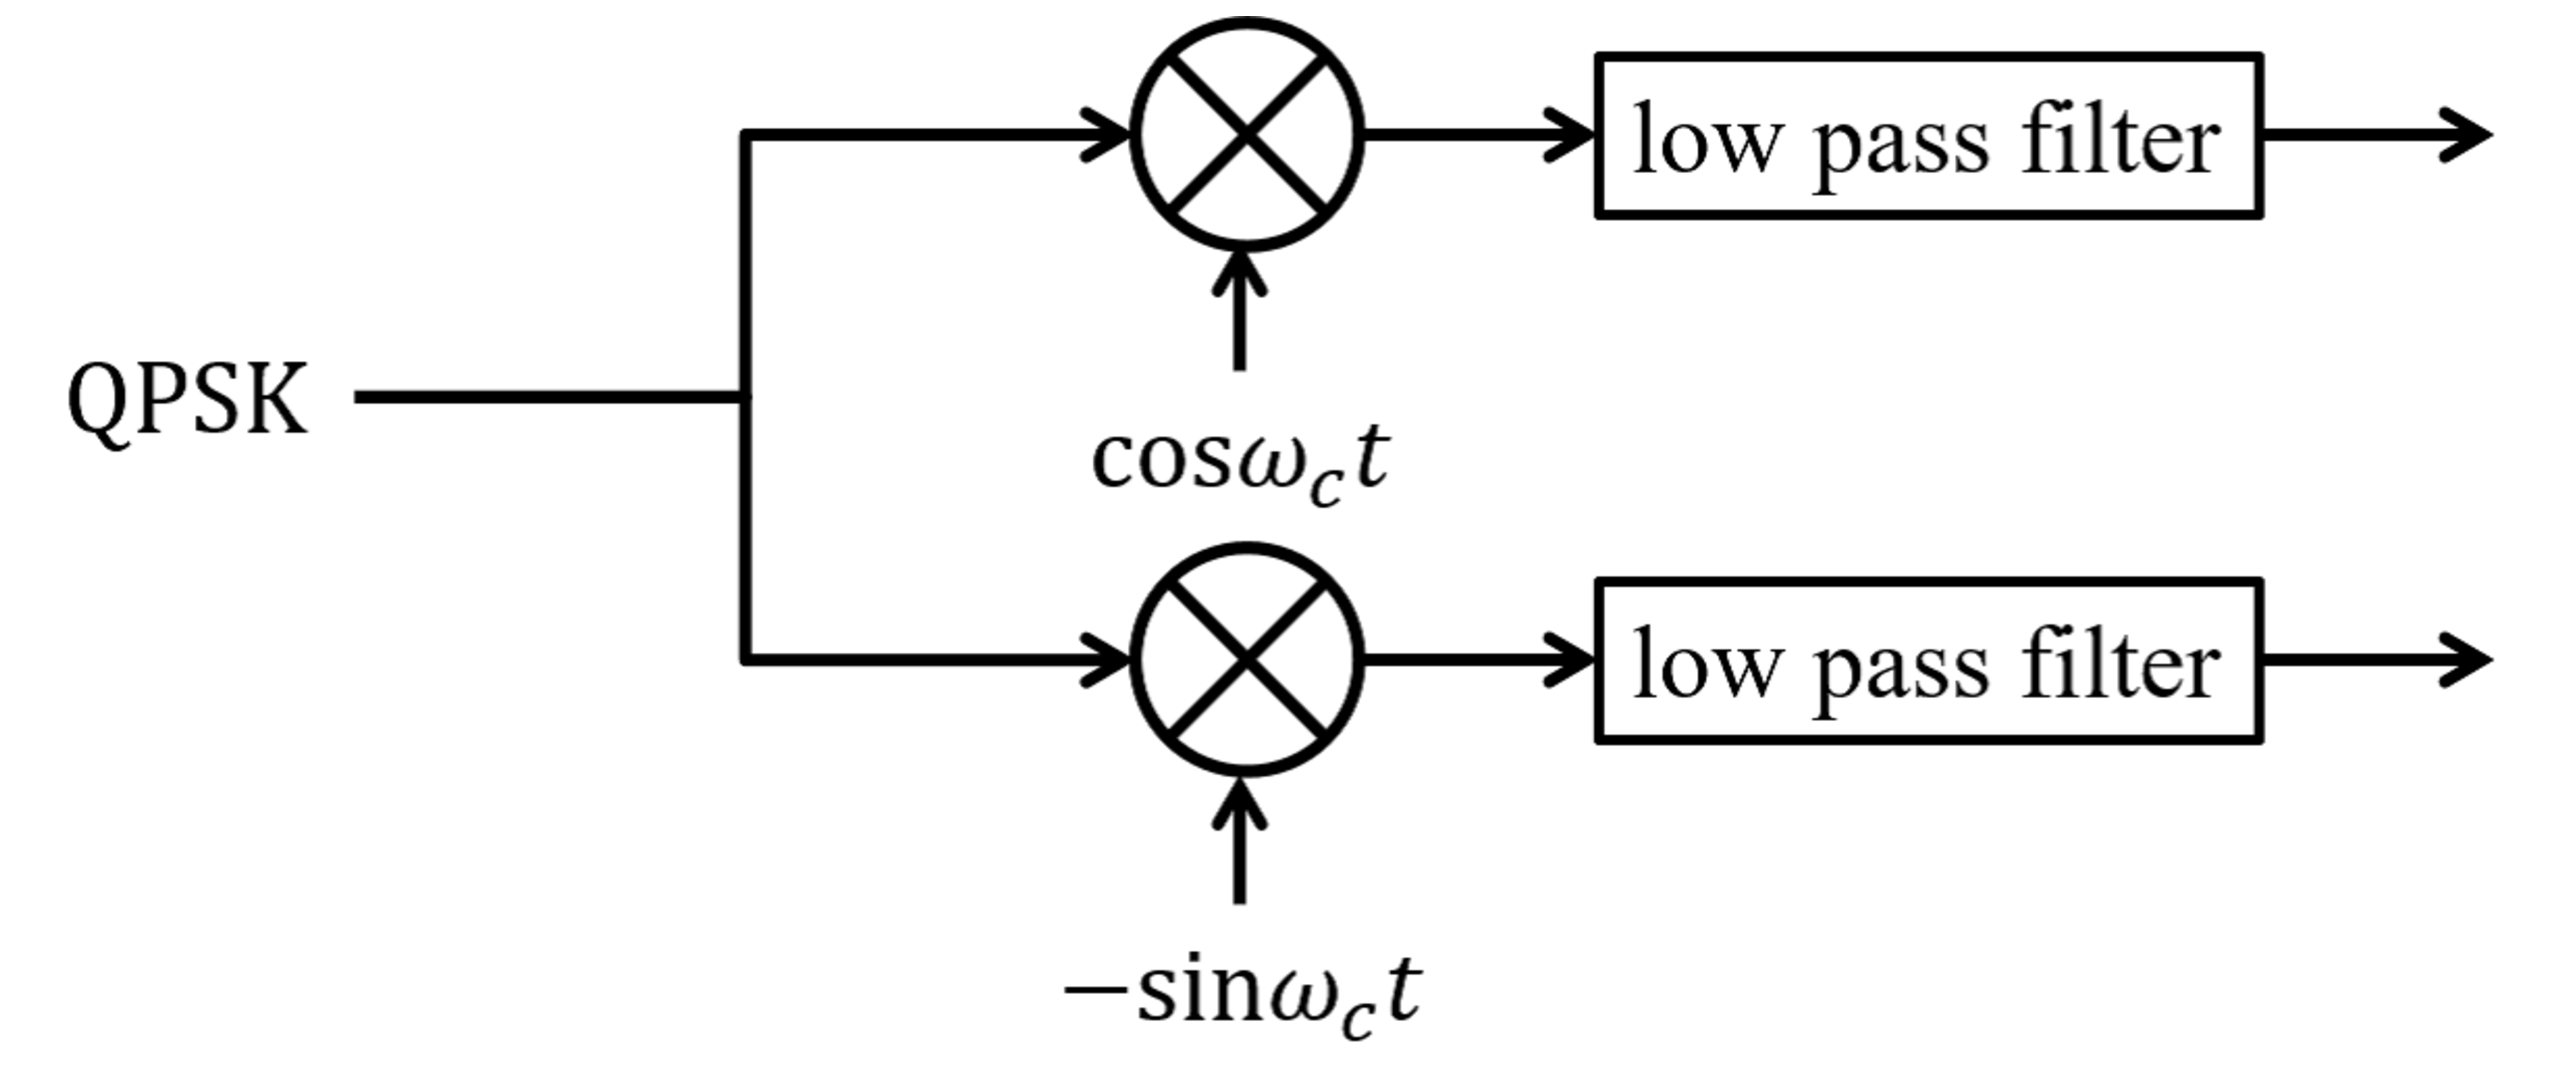
\includegraphics[scale = 0.25]{./chapter2/figure/douki.eps}
    \caption{QPSK変調の同期検波回路}
    \label{fig:qpskcoh}
  \end{center}
\end{figure}
%------------------------------------------------------------------

\subsection{信号の等価低域表現}
対象システムの特性をコンピュータシミュレーションのような離散時間処理によって評価する場合,サンプリング定理を満足するなるべく小さなサンプリング周波数を用い,演算量を削減することが望ましい.そこで本研究では,信号を複素ベースバンドで表現し,等価低域表現によるシミュレーションを行っている.

ここで,ベースバンド信号の帯域幅が$B[{\rm Hz}]$のQPSK変調信号を考える.搬送波の周波数が$f_c[{\rm Hz}]$である場合,信号の最高周波数が$f_c+B[{\rm Hz}]$となるため,標本化定理により,この信号は$2(f_c+B)[{\rm Hz}]$以上で標本化する必要がある.一方,式(\ref{eqqpsk})より,QPSK変調信号の複素数表現は,$\{Ad_1(t)+jAd_2(t)\}e^{j2\pi f_ct}$となる.複素数表現では,$f_c=0$として,複素ベースバンド信号で表すことができ,
\begin{eqnarray}
b(t)=Ad_1(t)+jAd_2(t)
\end{eqnarray}
となる.標本化定理から,$2B[{\rm Hz}]$以上でサンプリングすれば復調できるため,実信号表現の場合と比べてサンプリング周波数を低くすることができ,サンプル点数を減らすことができる.この表現方法を等価低域表現と呼ぶ\cite{takahata}.
%------------------------------------------------------------------------

\section{フェージング伝搬路の影響}
開空間を伝送媒体として用いる無線通信では,気象条件や地理的条件によってその伝搬路特性が変化する.
また,通信中に場所の移動が伴う場合は伝搬路特性の変動が更に厳しいものとなる.
この現象はフェージングと呼ばれ,送信信号に振幅変動や位相変動を発生させる.
その結果,受信信号の品質は顕著な影響を受ける \cite{saitou}.

\subsection{マルチパスフェージングの発生原理}
送信された電波は大気屈折率の変化や大地,山,建物,あるいは車等によって反射,回折,散乱する.
材質や入射角により,ある電波は大きな減衰を受け,ある電波はほとんど減衰せずに経路が変えられるなど
して,マルチパス伝搬路が形成される(図 \ref{fig:multipath}).

受信点では多数の波が干渉し,定在波が生じる.この中を移動すると到来する多数の波の干渉により
激しい振幅時間変動,位相時間変動が生じる.
この現象をフェージングと呼ぶ\cite{okumura}.
簡単な例として,複素搬送波$e^{j2\pi f_ct}$が伝送され,図 \ref{fig:coming_waves}のように,マルチパス伝搬路において複数の散乱波が受信される場合を考える.$n$番目のパスを通過した信号の振幅を$a_n(t)$,位相を$\theta_n(t)$とすれば,そのときの受信信号$r_n(t)$は,
\begin{eqnarray}
r_n(t)&=&{\rm Re}\left[a_n(t)e^{j2\pi f_c t+j\theta_n(t)}\right]\nonumber \\
&=&{\rm Re}\left[z_n(t)e^{j2\pi f_c t}\right]
\end{eqnarray}
となる.ここで$z_n(t)\equiv a_n(t)e^{j\theta_n(t)}$とし,$r_n(t)$の複素包絡線を表す.また,$a_n(t)$は複素包絡線$z_n(t)$の振幅変化,$\theta_n(t)$は複素包絡線$z_n(t)$の位相変化をそれぞれ表す.したがって,受信信号$r(t)$は,
\begin{eqnarray}
r(t)=\sum_{n=1}^{N}z_n(t)e^{j\pi f_ct}
\end{eqnarray}
となる.ここで,受信点や周囲の環境が静止している場合には,$a_n(t)$,$\theta_n(t)$はほとんど変化せず,準静的フェージングモデルを与える.一方,受信点が速度$v$で移動すると,到来角度$\phi_n$に応じて,$v\cos(\phi_n)/\lambda$のドップラー周波数変動を受け,動的フェージングモデルとなる.このとき,初期位相を$\varphi_n$とすると,$\theta_n(t)$は,
\begin{eqnarray}
\theta_n(t)=2\pi\frac{vt\cos\phi_n}{\lambda}+\varphi_n
\end{eqnarray}
となる.ここで,$v/\lambda=f_D$は最大ドップラー周波数といわれるものであり,物理的には移動局の進行方向($\phi_n=0$)からの到来波周波数が$f_D[{\rm Hz}]$だけ高くなるのに対して,後方($\phi_n=\pi$)からの到来波は$f_D[{\rm Hz}]$だけ低くなることを表す.
\begin{figure}[t]
  \begin{center}
    \includegraphics[scale = 0.25]{./chapter2/figure/multipaths.eps}
    \caption{マルチパス伝搬路モデル}
    \label{fig:multipath}
  \end{center}
\end{figure}

\begin{figure}[htbp]
	\begin{center}
		\includegraphics[scale=0.15]{./chapter2/figure/jushin.eps}
		\caption{マルチパス伝搬路の受信モデル}
		\label{fig:coming_waves}
	\end{center}
\end{figure}
%--------------------------------------------------------------------------------

\subsection{レイリーフェージング}
到来する素波数を$N$とする.このとき,受信信号$r(t)$の複素包絡線$z(t)$は,
\begin{eqnarray}
z(t)&=&\sum_{n=1}^{N}z_{n}(t) \nonumber \\
%&=&\sum_{n=1}^{N} a_{n}(t)e^{j\theta_{n}(t)} \nonumber \\
&=&\sum_{n=1}^{N}x_n(t)+j\sum_{n=1}^{N}y_n(t) \nonumber \\
&=& x(t)+j y(t)
\end{eqnarray}
となる.ここで,$x(t)$と$y(t)$はそれぞれ$z(t)$の同相成分,直交成分を表す.$x(t)$と$y(t)$は各波の強さが同程度である正弦波の和とすると,中心極限定理より$x(t)$,$y(t)$は平均値が0で等しい分散を持つ互いに独立な定常ガウス(Gauss)過程となる.$x=x(t)$,$y=y(t)$の結合確率密度関数$p(x,y)$は,
\begin{eqnarray}
p(x,y)=\frac{1}{2\pi \sigma^2}{\rm exp}\left(-\frac{x^2+y^2}{2\sigma^2}\right)
\end{eqnarray}
と表せる.ここで,$\sigma^2$は$r(t)$の平均受信電力である.包絡線振幅を$r$,位相を$\theta$とすると,
\begin{eqnarray}
\begin{cases}
r=\sqrt{x^2+y^2}& \\[4pt]
\theta=\tan^{-1}\left(\displaystyle \frac{y}{x}\right)&
\end{cases}
\end{eqnarray}
の関係がある.ここで,同相・直交成分の振幅が$(x, x+dx), (y, y+dy)$の領域に存在する確率は,デカルト座標から極座標に変換しても変わることはないため,次の式が成立する.
\begin{eqnarray}
\left\{
\begin{array}{ll}
p(x,y)dx\cdot dy & =p(r,\theta)dr\cdot d\theta  \\[12pt]
dx\cdot dy & =r\cdot dr\cdot d\theta
\end{array}
\right.
\end{eqnarray}
したがって,
\begin{eqnarray}
p(r,\theta)=\frac{r}{2\pi \sigma^2}{\rm exp}\left(-\frac{r^2}{2\sigma^2}\right)
\end{eqnarray}
となる.以上より,包絡線の確率密度関数$p(r)$と位相の確率密度関数$p(\theta)$は以下のように求められる.
\begin{eqnarray}
\left\{
\begin{array}{ll}
p(r)=\displaystyle \int_0^{2\pi}p(r,\theta)=\frac{r}{\sigma^2}{\rm exp}\left(-\frac{r^2}{2\sigma^2}\right)&(0\leq r \leq \infty)\\[12pt]
p(\theta)=\displaystyle \int_0^\infty p(r,\theta)dr=\frac{1}{2\pi} & (0\leq\theta\leq2\pi)
\end{array}
\right.
\end{eqnarray}
\begin{figure}[t]
	\begin{center}
		\includegraphics[scale=0.14]{./chapter2/figure/hourakusen.eps}
		\caption{包絡線と位相の確率密度関数}
		\label{figrayleigh}
	\end{center}
\end{figure}
$p(r)$,$p(\theta)$を図 \ref{figrayleigh}に示す.包絡線と位相の変動はそれぞれレイリー分布と一様分布に従うことがわかる.このようなフェージングをレイリーフェージングと呼ぶ\cite{saitou}\cite{okumura}.
%------------------------------------------------------------------------------ %基本的概念の解説
\chapter{Ping-Pong-Loopによる固有符号推定}
本章では,4章の検討内容の基礎となる,Ping-Pong-Loop(以下PPL)アルゴリズムについて説明する.

\section{Vector Coding}
最初にVCを説明するにあたって必要なチャネル行列の定義を行った上で,VCの概要について説明する.

\subsection{チャネル行列}
チャネルインパルス応答$h[n]$は以下で与えられている.
\begin{equation}
    h[n] = \left\{
        \begin{array}{ll}
            = 0 & (n<0 \quad or \quad n \geq K) \\
            \neq 0 & (n=0)
        \end{array}
    \right.
\end{equation}
伝送信号系列を$x[n]$とすると,受信信号系列$y[n]$は(3.1)式を用いて,次の畳み込み
演算で与えられる.
\begin{equation}
    y[n] = \sum_{m=0}^\infty h[n-m]x[m]
\end{equation}
送信変調ベクトルをN次の列ベクトル$\bm{X}(=x[0],x[1],\ldots,x[N-1])^T$,チャネル行列を
$\bm{H}$とすると,受信信号ベクトル$\bm{Y}$は(3.2)式を行列表記することで下記のように
与えられる.
\begin{equation}
    \bm{Y} = \bm{HX}
\end{equation}
ここで$\bm{Y}$は$M(=N+K-1)$次の列ベクトル$(=y[0],y[1],\ldots,y[M-1])^T$で,チャネル歪み
の影響でN次からM次になっている.Kはパス数である.$\bm{H}$はM行N列の行列で以下のように
表記される.
\begin{equation}
    \bm{H} = \left[
        \begin{array}{ccccc}
            h[0] & 0 & 0 & \ldots & 0 \\
            h[1] & h[0] & 0 & \ldots & 0 \\
            \vdots & h[1] & h[0] & \ldots & \vdots \\
            h[K-1] & \vdots & h[1] & \ldots & 0 \\
            0 & h[K-1] & \vdots & \ldots & h[0] \\
            0 & 0 & h[K-1] & \ldots & h[1] \\
            \vdots & \vdots & \vdots & \ldots & \vdots \\
            0 & 0 & 0 & \ldots & h[K-1]
        \end{array}
    \right]
\end{equation}

次にチャネル行列$\bm{H}$に対するMFが$\bm{H^H}$であることを示す.SNRを最大とするMFの
インパルス応答を$h_{MF}[n]$とする.$h[n]$と$h_{MF}[n]$を接続した連結システムのインパルス応答
$h^{\prime}[n]$は,次の畳み込み演算で与えられる.
\begin{equation}
    h^{\prime}[n] = \sum_{m=0}^{\infty} h[m]h_{MF}[n-m]
\end{equation}
(3.5)式において,$n=0$のときがSNR最大であり,その出力は,
\begin{equation}
    h^{\prime}[0] = \sum_{m=0}^{K-1} |h[m]|^2
\end{equation}
(3.6)式の畳み込み演算を行列表記すると,$\bm{H^{\prime}}=\bm{H_{MF}H}$となる.簡単のため,$N=3$,$K=2$
での$\bm{H}$を考え,$\bm{H_{MF}=\bm{H^H}}$として$\bm{H^{\prime}}$を計算,さらにこの$\bm{H^{\prime}}$
にインパルス$\bm{I}=(1 \quad 0 \quad 0)^T$を入力したときの出力を計算すると,
\begin{eqnarray}
    \bm{H^{\prime}}I &=& \left[
        \begin{array}{ccc}
            |h[0]|^2+|h[1]|^2 & h^*[1]h[0] & 0 \\
            h^*[0]h[1] & |h[0]|^2+|h[1]|^2 & h^*[1]h[0] \\
            0 & h^*[0]h[1] & |h[0]|^2+|h[1]|^2
        \end{array}
    \right]
    \left[
        \begin{array}{c}
            1 \\
            0 \\
            0
        \end{array} 
    \right] \nonumber \\
    &=& \left[
        \begin{array}{c}
            |h[0]|^2+|h[1]|^2 \\
            h^*[0]h[1] \\
            0
        \end{array}
    \right]
\end{eqnarray}
(3.7)式の1行1列に着目すると,
\begin{equation}
    |h[0]|^2+|h[1]|^2 = \sum_{m=0}^{2-1} |h[m]|^2 \nonumber
\end{equation}
であり,これは先に述べたSNR最大時の出力である.以上より,$\bm{H^H}$が$\bm{H}$に対するMFで
あることが分かる.

\subsection{合成チャネル行列}
従来のVCでは,最初にチャネル行列$\bm{H}$の推定を行う.そして推定した$\bm{H}$から$\bm{H^H}$を求める.
$\bm{H^H}$とは$\bm{H}$の随伴行列(共役転置行列)であると同時に,$\bm{H}$に対するMFである(2.4.1).
VCの拡散符号には
$\bm{H}$と$\bm{H^H}$を接続した合成チャネル行列$\bm{H^HH}$の固有符号を利用している.$\bm{H^HH}$は
エルミート行列となっており,2.2節で説明した(性質3)により,$\bm{H^HH}$の固有符号を拡散符号として
用いることでISIの発生を防ぐことができる.以下では$\bm{H^HH}$がエルミート行列であることを示す.
簡単のため,$N=3$,$K=2$での$\bm{H}$を考える.

\begin{equation}
    H = \left[
        \begin{array}{ccc}
            h[0] & 0 & 0 \\
            h[1] & h[0] & 0 \\
            0 & h[1] & h[0] \\
            0 & 0 & h[1]
        \end{array}
    \right]
\end{equation}

(3.8)式$\bm{H}$の随伴行列(共役転置行列)である$\bm{H^H}$は,

\begin{equation}
    H^H = \left[
        \begin{array}{cccc}
            h[0]^* & h[1]^* & 0 & 0 \\
            0 & h[0]^* & h[1]^* & 0 \\
            0 & 0 & h[0]^* & h[1]^* \\
        \end{array}
    \right]
\end{equation}

(3.8)式,(3.9)式から $\bm{H^HH}$を計算すると,

\begin{equation}
    H^HH = \left[
        \begin{array}{ccc}
            |h[0]|^2+|h[1]|^2 & h[1]^*h[0] & 0 \\
            h[0]^*h[1] & |h[0]|^2+|h[1]|^2 & h[1]^*h[0] \\
            0 & h[0]^*h[1] & |h[0]|^2+|h[1]|^2 \\
        \end{array}
    \right]
\end{equation}

明らかに,$\bm{H^HH=(H^HH)^H}$となっており,エルミート行列の定義(2.2)により,
$\bm{H^H}$はエルミート行列であると言える.

\subsection{VC計算過程}
図\ref{figVC}はVCでの伝送を表すブロック図である.図\ref{figVC}の送信側から伝送される送信変調ベクトル
$\bm{X}$は次の式で与えられる.

\begin{equation}
    \bm{X} = \sum_{i=0}^{N-1} S_i\bm{e_i}
\end{equation}

ここで,$S_i$は伝送する情報シンボル,$\bm{e_i}$は拡散符号として用いている$\bm{H^HH}$の
固有符号群である.受信信号ベクトル$\bm{Y}$は,$\bm{X}$がチャネルを通過し,これに雑音が
加わったものである.

\begin{equation}
    \bm{Y} = \bm{HX}+\bm{n} = \sum_{i=0}^{N-1} S_i\bm{H_ie_i}+\bm{n}
\end{equation}

この$\bm{Y}$は受信機入力点での受信信号ベクトルであり,最終的な受信信号ベクトル$\bm{Y^{\prime}}$
はチャネルに対するMF($\bm{H^H}$)通過後の$\bm{Y}$である.

\begin{equation}
    \bm{Y^{\prime}}=\bm{H^HY}=\bm{H^H}
    \left(
        \sum_{i=0}^{N-1} S_i\bm{H_ie_i}+\bm{n}
    \right)
    =\sum_{i=0}^{N-1} \lambda_iS_i\bm{e_i}+\bm{H^Hn}
\end{equation}

ここで,$\lambda_i$は$\bm{H^HH}$の固有値である.なお,(2.32)式では,$\bm{H^HHe}=\lambda\bm{e}$
という行列とその行列の固有値・固有符号との関係を用いている.
ここから拡散符号(固有符号$\bm{e}$)の直交性を利用し,ISIの影響を受けずに情報シンボルを
取り出すことができる.方法としては,例えばk番目の情報シンボル$S_k$を求める場合,k番目の
拡散符号(固有符号$\bm{e_k}$)と(2.32)式との内積を計算する.

\begin{equation}
    \bm{e_k^HY^{\prime}}=\bm{e_k^H}.
    \left(
        \sum_{i=0}^{N-1} \lambda_iS_i\bm{e_k}+\bm{H^Hn}
    \right)
    =\lambda_kS_k+(\bm{He_k})^H\bm{n}
\end{equation}

(2.33)式の第1項は$S_k$のk番目の固有値(実数)倍であることから直交符号分割が実現できていることが
分かる.(2.33)式の第2項は処理できずに残ってしまった雑音である.

\begin{figure}
    \centering
    \includegraphics[width=\linewidth]{chapter3/figure/VC.eps}
    \caption{VC概略図}
    \label{figVC}
\end{figure}

\section{PPL(Ping-Pong-Loop)}
従来のVCでは,伝搬路推定を用いて伝搬路行列$\bm{H}$を求めた後,そこから合成チャネル行列
$\bm{H^HH}$を計算し,当該チャネル行列を固有値分解することによって固有値・固有ベクトルを求める.
PPLは,従来の伝搬路推定,固有値分解の演算部分を二つの無線機間のごく単純な往復処理に置き換えた
ものである.
PPLの原理は,行列の固有値・固有ベクトルの導出方法として一般的なべき乗法を基礎とする.
任意ベクトル$\bm{x}$を,二つの無線機間で繰り返し送受信しつつ,各無線機に
おいて簡単な非線形処理を施すことで,徐々にこの任意ベクトル$\bm{x}$を固有ベクトルへと収束させる.
PPLは,伝搬路推定や固有値分解等の膨大な演算をごく単純な非線形処理を含む送受信機間往復に置換する
点を特徴とする.

PPLの例として,無線機Aと無線機B間での反復処理を考える.
ここでは上下回線とも同一周波数を用いる.
半2重通信を想定する.また,伝搬路行列$\bm{H}$は時不変チャネルとし,雑音の影響はないとする.
PPLを大きく分けて,無線機Aから無線機Bへの往路と無線機Bから無線機Aへの復路の二つに分けて説明する.
無線機A,B間の往復によって,任意ベクトル$\bm{x}$が合成チャネル行列$\bm{H^H}$を通過したと
見做すことができれば,2.3節で解説したべき乗法のアルゴリズムによって伝搬路推定を用いることなく
固有値・固有ベクトルを求めることが可能になる.
図\ref{figPPL}にPPLの概略図を示す.

\begin{figure}
    \centering
    \includegraphics[width=\linewidth]{chapter3/figure/PPL.eps}
    \caption{PPL概略図}
    \label{figPPL}
\end{figure}

まず,往路について,無線機Aから任意ベクトル$\bm{x}$を送信する.当該ベクトルは伝搬路$\bm{H}$を
通過し,無線機Bの受信端にて$\bm{Hx}$として受信される.
次に,復路について,$\bm{Hx}$を無線機Aへと伝送するが,この時,復路の伝搬路が$\bm{H^H}$と
等価となるように,伝送の前後に非線形処理Iと非線形処理Jの二つを挿入する.
これによって,無線機A,B間を反復することで,見かけ上,任意ベクトル$\bm{x}$が
合成チャネル行列$\bm{H^HH}$を通過したと見做すことができるようになる.
一連の反復処理を複数回繰り返すことで,べき乗法の原理に基づいて任意ベクトル$\bm{x}$は徐々に
固有ベクトルに収束していき,その過程で固有値も求めることができる.

\section{PPLにおける両送信機での非線形処理}
本節では,3.2節で述べた復路のチャネルを$\bm{H^H}$と見做すための非線形処理I,Jについて説明する.
図 \ref{figPPL}が示すように,無線機Aの非線形処理を処理J,無線機Bの非線形処理を処理Iとする.
具体的に,非線形処理I,Jによって,どのようにして合成チャネル行列$\bm{H^HH}$を通過したと見做せるか
解説する.
説明に当たって,以下では$N=3$の任意ベクトル$\bm{x}$,パス数$K=3$の$\bm{H}$を考える.
図 \ref{figProcI}と図 \ref{figProcJ}にそれぞれ処理I、処理Jの手順を示す.

\begin{figure}
    \centering
    \includegraphics[width=0.6\linewidth]{chapter3/figure/ProcI.eps}
    \caption{処理I}
    \label{figProcI}
\end{figure}
\begin{figure}
    \centering
    \includegraphics[width=0.7\linewidth]{chapter3/figure/ProcJ.eps}
    \caption{処理J}
    \label{figProcJ}
\end{figure}

図 \ref{figProcI}に示している通り,処理Iはベクトルの複素共役をとった後,上下を反転させる.
また,処理Jは図 \ref{figProcJ}にあるように途中まで処理Iと同じプロセスとなっているが,これに
加えて最後にベクトルの上下から(K-1)個分の要素を除去する処理が追加されている.

次に,処理I,処理Jを施すことでどのようにして復路を$\bm{H^H}$と見做せるようになるのかを具体例を
使って説明する.
説明に当たって,伝送する任意ベクトル$\bm{x}$,伝搬路行列$\bm{H}$は以下を考える.

\begin{equation}
    \bm{x} = \left[
        \begin{array}{c}
            x_0 \\
            x_1 \\
            x_2
        \end{array}
    \right]
\end{equation}

\begin{equation}
    \bm{H} = \left[
        \begin{array}{ccc}
            h[0] & 0 & 0 \\
            h[1] & h[0] & 0 \\
            h[2] & h[1] & h[0] \\
            0 & h[2] & h[1] \\
            0 & 0 & h[2]
        \end{array}
    \right]
\end{equation}

まず,$\bm{x}$が無線機Aから無線機Bに向けて伝送される場合を考える.
伝搬路$\bm{H}$を通って無線機Bの受信端で受信されたベクトル$\bm{x^{\prime}}$は,
\begin{equation}
    \bm{x^{\prime}} = \bm{Hx} = \left[
        \begin{array}{c}
            h[0]x_0 \\
            h[1]x_0 + h[0]x_1 \\
            h[2]x_0 + h[1]x_1 + h[0]x_2 \\
            h[2]x_1 + h[1]x_2 \\
            h[2]x_2
        \end{array}
    \right]
    = \left[
        \begin{array}{c}
            x_0^{\prime} \\
            x_1^{\prime} \\
            x_2^{\prime} \\
            x_3^{\prime} \\
            x_4^{\prime}
        \end{array}
    \right]
\end{equation}
となる.このベクトル$\bm{x^{\prime}}$に処理Iを施すと,
\begin{equation}
    \bm{x^{\prime}} = \bm{Hx} = \left[
        \begin{array}{c}
            h[2]^*x_2^* \\
            h[2]^*x_1^* + h[1]^*x_2^* \\
            h[2]^*x_0^* + h[1]^*x_1^* + h[0]^*x_2^* \\
            h[1]^*x_0^* + h[0]^*x_1^* \\
            h[0]^*x_0^*
        \end{array}
    \right]
    = \left[
        \begin{array}{c}
            x_4^{\prime*} \\
            x_3^{\prime*} \\
            x_2^{\prime*} \\
            x_1^{\prime*} \\
            x_0^{\prime*}
        \end{array}
    \right]
\end{equation}
となる.これを復路の伝搬路$\bm{H}$に通すと,無線機Aの受信端で受信されるベクトルは,
\begin{equation}
    \bm{Hx^{\prime*}} \left[
        \begin{array}{c}
            h[0]x_4^{\prime*} \\
            h[1]x_4^{\prime*}+h[0]x_3^{\prime*} \\
            h[2]x_4^{\prime*}+h[1]x_3^{\prime*}+h[0]x_2^{\prime*} \\
            h[2]x_3^{\prime*}+h[1]x_2^{\prime*}+h[0]x_1^{\prime*} \\
            h[2]x_2^{\prime*}+h[1]x_1^{\prime*}+h[0]x_0^{\prime*} \\
            h[2]x_1^{\prime*}+h[1]x_0^{\prime*} \\
            h[2]x_0^{\prime*}
        \end{array}
    \right]
\end{equation}
となり,処理Jを施すと,
\begin{equation}
    \left[
        \begin{array}{c}
            h[2]^*x_2^{\prime}+h[1]^*x_1^{\prime}+h[0]^*x_0^{\prime} \\
            h[2]^*x_3^{\prime}+h[1]^*x_2^{\prime}+h[0]^*x_1^{\prime} \\
            h[2]^*x_4^{\prime}+h[1]^*x_3^{\prime}+h[0]^*x_2^{\prime}
        \end{array}
    \right]
\end{equation}
となる.

次に,無線機Bで受信された$\bm{x^{\prime}}$に$\bm{H^H}$をかけたものが,式(3.20)と一致するか
確認する.まず,伝搬路行列$\bm{H}$の随伴行列$\bm{H^H}$は次のようになる.
\begin{equation}
    \bm{H^H} = \left[
        \begin{array}{ccccc}
            h[0]^* & h[1]^* & h[2]^* & 0 & 0 \\
            0 & h[0]^* & h[1]^* & h[2]^* & 0 \\
            0 & 0 & h[0]^* & h[1]^* & h[2]^*
        \end{array}
    \right]
\end{equation}

これを無線機Bで受信された$\bm{x^{\prime}}$に左からかけると,
\begin{equation}
    \bm{H^Hx^{\prime}} = \left[
        \begin{array}{c}
            h[2]^*x_2^{\prime}+h[1]^*x_1^{\prime}+h[0]^*x_0^{\prime} \\
            h[2]^*x_3^{\prime}+h[1]^*x_2^{\prime}+h[0]^*x_1^{\prime} \\
            h[2]^*x_4^{\prime}+h[1]^*x_3^{\prime}+h[0]^*x_2^{\prime}
        \end{array}
    \right]
\end{equation}
となり,これは式(3.20)と一致する.よって,非線形処理IとJを施すことで復路を見かけ上$\bm{H^H}$と
見做せることが確認できた.

\section{PPLにおける第1固有ベクトル導出}
ここではべき乗法を基本原理として,PPLにおいてどのようにして合成チャネル行列の固有ベクトル・固有値が
求められていくか解説を行う.まず,3.3節で示したように二つの無線機間で任意ベクトル$\bm{x}$を往復せた時,
非線形処理によって1往復後のベクトルは$\bm{H^HHx}$となる.これによって,べき乗法の
適用が可能になり,複数回$\bm{H^HH}$をかけることで2.3節で解説したように徐々に$\bm{x}$が第一固有ベクトル
へと収束していく.

具体的な数式を用いて,PPLにおいてどのように第一固有ベクトルが求められていくか見ていく.
合成チャネル行列$\bm{H^HH}$の固有値の大きさは$|\lambda_1|>|\lambda_2|>\ldots>|\lambda_M|$の
関係があるとして,また,これに対応する固有ベクトルを$\bm{u_1},\bm{u_2},\ldots,\bm{u_M}$とする.
図 \ref{figProcIJ1}に第1固有ベクトル導出の概略図を示す.
\begin{figure}
    \centering
    \includegraphics[width=0.7\linewidth]{chapter3/figure/ProcIJ1.eps}
    \caption{第1固有ベクトル導出}
    \label{figProcIJ1}
\end{figure}

まず,任意ベクトル$\bm{x}$を一対の無線機間で1往復させた場合を考える.
ここで,任意ベクトル$\bm{x}$は2.1.3節より,固有符号群$\bm{u_1},\bm{u_2},\ldots,\bm{u_M}$と
定数$c_1,c_2,\ldots,c_M$により表すことができることに留意する.
無線機間を1往復させ$\bm{x}$に$\bm{H^HH}$がかかったベクトルは,
\begin{eqnarray}
    \bm{H^HHx} &=& \bm{H^HH}\sum_{i=1}^M c_i\bm{u_i} \nonumber \\
    &=& \sum_{i=1}^M c_i\lambda_i\bm{u_i} \hspace{10mm} (\because \bm{H^HHu_i}=\lambda_i\bm{u_i}) \nonumber \\
    &=& \lambda_1\left(
        c_1\bm{u_1}+\frac{\lambda_2}{\lambda_1}c_2\bm{u_2}+\ldots+\frac{\lambda_M}{\lambda_1}c_M\bm{u_M}
    \right)
\end{eqnarray}
となる.次に,2往復目に移るのだが,1往復後のベクトルをそのまま繰り替えし往復させていくと,ベクトルの大きさが無限に増大
していってしまうため,往復ごとに正規化をする必要がある.
正規化は,ベクトルの大きさでベクトル全体を除算する処理なので,n往復後の正規化処理は,
\begin{equation}
    N_n = \sqrt{(\lambda_1^nc_1)^2+(\lambda_2^nc_2)^2+\cdots+(\lambda_M^nc_M)^2}
\end{equation}
で除算することになる.よって,1往復時の正規化処理後のベクトルは,
\begin{equation}
    \frac{1}{N_1}\lambda_1\left(
        c_1\bm{u_1}+\frac{\lambda_2}{\lambda_1}c_2\bm{u_2}+\ldots+\frac{\lambda_M}{\lambda_1}c_M\bm{u_M}
    \right)
\end{equation}
となる.2往復後のベクトルは,
\begin{eqnarray}
    \bm{H^HH(H^HHx)} &=& \bm{H^HH}\sum_{i=1}^M c_i\lambda_i\bm{u_i} \nonumber \\
    &=& \sum_{i=1}^M c_i\lambda_i^2\bm{u_i} \nonumber \\
    &=& \lambda_1^2\left(
        c_1\bm{u_1}+\frac{\lambda_2}{\lambda_1^2}c_2\bm{u_2}+\ldots+\frac{\lambda_M}{\lambda_1^2}c_M\bm{u_M}
    \right)
\end{eqnarray}
となり,正規化を行うと,
\begin{equation}
    \frac{1}{N_2}\lambda_1^2\left(
        c_1\bm{u_1}+\frac{\lambda_2^2}{\lambda_1^2}c_2\bm{u_2}+\ldots+\frac{\lambda_M^2}{\lambda_1^2}c_M\bm{u_M}
    \right)
\end{equation}
となる.以上のように繰り返し往復処理を行っていくと,n回往復時の正規化後ベクトルは,
\begin{eqnarray}
    \frac{1}{N_n}\lambda_1^n\left(
        c_1\bm{u_1}+\frac{\lambda_2^n}{\lambda_1^n}c_2\bm{u_2}+\ldots+\frac{\lambda_M^n}{\lambda_1^n}c_M\bm{u_M}
    \right)
\end{eqnarray}
と表せる.固有値には,$\bm{\lambda_1},\bm{\lambda_2},\ldots,\bm{\lambda_M}$の関係があるため,nが十分大きい時,
\begin{equation}
    \frac{\lambda_i}{\lambda_1} \simeq 0 \hspace{10mm} (i=2,3,\ldots,M)
\end{equation}
であるので,(3.28)式の第2項以降は0となる.よって,n往復後のベクトルは,
\begin{eqnarray}
    \frac{1}{N_n}\lambda_1^n\left(
        c_1\bm{u_1}+\frac{\lambda_2^n}{\lambda_1^n}c_2\bm{u_2}+\ldots+\frac{\lambda_M^n}{\lambda_1^n}c_M\bm{u_M}
    \right) &\simeq& \frac{1}{N_n}\lambda_1^nc_1\bm{u_1} \nonumber \\
    &=& \frac{\lambda_1^nc_1\bm{u_1}}{\sqrt{(\lambda_1^nc_1)^2+(\lambda_2^nc_2)^2+\cdots+(\lambda_M^nc_M)^2}} \nonumber \\
    &=& \frac{c_1\bm{u_1}}{\sqrt{ c_1^2 + \left(\frac{\lambda_2}{\lambda_1}\right)^{2n}c_2^2+\left(\frac{\lambda_3}{\lambda_1}\right)^{2n}c_3^2+\cdots+\left(\frac{\lambda_M}{\lambda_1}\right)^{2n}c_M^2}} \nonumber \\
    &\simeq& \frac{c_1\bm{u_1}}{c_1} \nonumber \\
    &=& \bm{u_1}
\end{eqnarray}
となる.なお,3行目の分母の第2項以降も固有値の大小関係より0となっている.

以上より,複数回無線機間往復を繰り返すことによって第一固有ベクトルが求められることが
確認できた.また,固有値については,
\begin{equation}
    \lambda_1 = \frac{\bm{H^HHu_1}}{\bm{u_1}} = \frac{\lambda_1\bm{u_1}}{\bm{u_1}}
\end{equation}
として,往復後のベクトルを往復前のベクトルで除算することで求められる.

\section{PPLにおける第2固有ベクトル以降導出}
第一固有値・固有ベクトルの導出については前節で解説したとおりだが,実際のVCでは第2固有値・固有ベクトル以降
も必要となる.ここでは,第2以降の固有値・固有ベクトルが獲得される様子を見ていく.

まず,2.2節のスペクトル定理より,合成チャネル行列$\bm{H^HH}$は,
\begin{equation}
    \bm{H^HH} = \lambda_1\bm{u_1u_1^H}+\lambda_2\bm{u_2u_2^H}+\ldots+\lambda_M\bm{u_Mu_M^H}
\end{equation}
と書ける.(3.32)式の右辺第1項を左辺に移項すると,
\begin{equation}
    (\bm{H^HH})^{\prime}=\bm{H^HH}-\lambda_1\bm{u_1u_1^H}=\lambda_2\bm{u_2u_2^H}+\ldots+\lambda_M\bm{u_Mu_M^H}
\end{equation}
となる.第2固有ベクトルは,この$(H^HH)^{\prime}$に対してべき乗法を適用することで求めることができる.
しかし,当然ながら実際の合成チャネル行列は$\bm{H^HH}-\lambda_1\bm{u_1u_1^H}$のような形には
なっていないので,適当な式変形を行うことでこれを実現しなければならない.
この様子を具体的に見ていく.
図 \ref{figProcIJ2}に第2固有ベクトル導出の概略図を示す.
\begin{figure}
    \centering
    \includegraphics[width=0.7\linewidth]{chapter3/figure/ProcIJ2.eps}
    \caption{第2固有ベクトル導出}
    \label{figProcIJ2}
\end{figure}

まず,単純に1往復した後に,前節で解説したようにこの時点での固有ベクトル$\bm{u_1}$を求める.
\begin{equation}
    \bm{u_1} = \frac{1}{N_1}\bm{H^HHx}
\end{equation}
次に,見かけ上(3.33)式のような$(\bm{H^HH})^{\prime}$を通過したとみなせるよう,
1往復後に得られるベクトル$\bm{H^HHx}$から$\lambda_1\bm{u_1u_1^Hx}$を減算すると,
\begin{eqnarray}
    \bm{H^HHx}-\lambda_1\bm{u_1u_1^Hx} &=& \bm{H^HH}\sum_{i=1}^M c_i\bm{u_i}-\lambda_1\bm{u_1u_1^H}\sum_{i=1}^M c_i\bm{u_i} \nonumber \\
    &=& \sum_{i=1}^M c_i\lambda_i\bm{u_i}-\sum_{i=1}^M c_i\lambda_1\bm{u_1u_1^H}\bm{u_i} \nonumber \\
    &=& \sum_{i=1}^M c_i\lambda_i\bm{u_i}-c_1\lambda_1\bm{u_1} \hspace{10mm} (\because 固有ベクトルの直交性) \nonumber \\
    &=& \sum_{i=2}^M c_i\lambda_i\bm{u_i} \nonumber \\
    &=& \lambda_2\left(
        c_2\bm{u_2} + \frac{\lambda_3}{\lambda_2}c_3\bm{u_3} + \cdots + \frac{\lambda_M}{\lambda_2}c_M\bm{u_M}
    \right)
\end{eqnarray}
となる.これを$M_n$(nは往復数),
\begin{equation}
    M_n = \sqrt{(\lambda_2^nc_2)^2+(\lambda_3^nc_2)^2+\cdots+(\lambda_M^nc_M)^2}
\end{equation}
で正規化すると,
\begin{equation}
    \frac{1}{M_1}\lambda_2\left(
        c_2\bm{u_2} + \frac{\lambda_3}{\lambda_2}c_3\bm{u_3} + \cdots + \frac{\lambda_M}{\lambda_2}c_M\bm{u_M}
    \right)
\end{equation}
となる.n回往復後のベクトルを同様にして表記した場合,
\begin{eqnarray}
    (\bm{H^HH})^n\bm{x}-\lambda_1^n\bm{u_1u_1^Hx} &=& (\bm{H^HH})^n\sum_{i=1}^M c_i\bm{u_i}-\lambda_1^n\bm{u_1u_1^H}\sum_{i=1}^M c_i\bm{u_i} \nonumber \\
    &=& \sum_{i=1}^M c_i\lambda_i^n\bm{u_i}-\sum_{i=1}^M c_i\lambda_1^n\bm{u_1u_1^H}\bm{u_i} \nonumber \\
    &=& \sum_{i=1}^M c_i\lambda_i^n\bm{u_i}-c_1\lambda_1^n\bm{u_1} \hspace{10mm} (\because 固有ベクトルの直交性) \nonumber \\
    &=& \sum_{i=2}^M c_i\lambda_i^n\bm{u_i} \nonumber \\
    &=& \lambda_2^n\left(
        c_2\bm{u_2} + \left(\frac{\lambda_3}{\lambda_2}\right)^nc_3\bm{u_3} + \cdots + \left(\frac{\lambda_M}{\lambda_2}\right)^nc_M\bm{u_M}
    \right)
\end{eqnarray}
と表される.これを正規化すると,
\begin{equation}
    \frac{1}{M_n}\lambda_2^n\left(
        c_2\bm{u_2} + \left(\frac{\lambda_3}{\lambda_2}\right)^nc_3\bm{u_3} + \cdots + \left(\frac{\lambda_M}{\lambda_2}\right)^nc_M\bm{u_M}
    \right)
\end{equation}
となる.ここで,固有値の大小関係$|\lambda_1|>|\lambda_2|>\ldots>|\lambda_M|$より,
nが十分に大きい場合,(3.39)式の右辺第2項以降は0に近似されるので,
\begin{eqnarray}
    \frac{1}{M_n}\left((\bm{H^HH})^n\bm{x}-\lambda_1^n\bm{u_1u_1^Hx}\right) &\simeq& \frac{1}{M_n}\lambda_2^nc_2\bm{u_2} \nonumber \\
    &=& \frac{\lambda_2^nc_2\bm{u_2}}{\sqrt{(\lambda_2^nc_2)^2+(\lambda_3^nc_2)^2+\cdots+(\lambda_M^nc_M)^2}} \nonumber \\
    &=& \frac{c_2\bm{u_2}}{\sqrt{c_2^2 + \left(\frac{\lambda_3}{\lambda_2}\right)^{2n}c_3^2+\left(\frac{\lambda_4}{\lambda_2}\right)^{2n}c_4^2+\cdots+\left(\frac{\lambda_M}{\lambda_2}\right)^{2n}c_M^2}} \nonumber \\
    &\simeq& \frac{c_2\bm{u_2}}{c_2} \nonumber \\
    &=& \bm{u_2}
\end{eqnarray}
このように第2固有ベクトル$\bm{u_2}$が求められる.よって,第2固有ベクトルがべき乗法によって
求められることが確かめられた.第3固有符号以降も同様に,
\begin{equation}
    (\bm{H^HH})^{\prime} = \bm{H^HH}-\lambda_1\bm{u_1u_1^H}-\lambda_2\bm{u_2u_2^H}=\lambda_3\bm{u_3u_3^H}+\ldots+\lambda_M\bm{u_Mu_M^H}
\end{equation}
を通過したとみなせるように,求めた$\bm{u_1,u_2}$からなる式を適当に減算することで求めることができる.
以上の一連の反復処理をPPLアルゴリズムと呼ぶ. %PPLアルゴリズム解説
\chapter{BER理論値を指標とする送信電力制御適用型使用チャネル足切りアルゴリズム
}

\section{研究背景}

\section{検討内容}
\subsection{BER理論値を指標とする使用チャネル足切りアルゴリズム}
\subsection{送信電力制御を用いたBER理論値最小化}
\subsection{送信電力制御適用時の使用チャネル足切りアルゴリズム}

\section{検証}
\subsection{BER理論値を指標とする使用チャネル足切りアルゴリズム}
\subsubsection{シミュレーション諸元}
\subsubsection{シミュレーション結果}
\subsection{送信電力制御を用いたBER理論値最小化}
\subsubsection{シミュレーション諸元}
\subsubsection{シミュレーション結果}
\subsection{送信電力制御適用時の使用チャネル足切りアルゴリズム}
\subsubsection{シミュレーション諸元}
\subsubsection{シミュレーション結果}
 %提案手法解説・検証
\chapter{まとめ}
VCは,伝搬路と伝搬路の整合フィルタからなる合成チャネル行列の固有ベクトルを拡散符号と
するCDMである.
VCの拡散符号は,合成チャネル行列のエルミート性から互いに直交性を示す.すなわち,
送受信機において拡散・逆拡散処理を施すことによって,シンボル間干渉(ISI)を
生じさせることなく各変調信号を取り出すことが可能である.
また,受信機側に伝搬路に対する整合フィルタを置くことで,遅延派の取りこぼしのない
パスダイバーシチを実現することができる.この点において,遅延派の影響を削除する
OFDMと比較して優れた伝送特性を示すとされている.
固有ベクトルの獲得については,これまで伝搬路推定による方法が検討されて
きた.従来の方法では,まず伝搬路推定によって正確な伝搬路情報を獲得する必要が
あることと,伝搬路行列から合成チャネル行列の計算を行った後に,固有値分解に
よって固有ベクトルを求める必要があり,膨大な計算量が必要となる.

チャネル推定を用いる手法に対して,伝搬路推定や固有値分解の演算に代わって,
ごく簡単な非線形処理と無線機間反復処理によって逐次的に固有ベクトルを獲得する,
PPL(Ping-Pong-Loop)という手法が存在する.
PPLは,演算能力の低い無線機でも簡単な無線機間反復処理によって固有ベクトルを
獲得することができる点をメリットとしているが,現状のアルゴリズムでは
多くの無線機間反復数を必要とするという課題があった.また,VC自体の課題として,
固有ベクトルに対応する固有値がチャネルの利得になることから,固有値が小さい
チャネルにおいて伝送する情報の誤り率が高くなってしまうという課題があった.

本論文ではこれらの問題の解決方法として以下の内容について検討を行った.
\begin{enumerate}
    \item 通信品質が基準以下である固有ベクトルに関してPPLの反復処理を停止する,固有ベクトル足切りアルゴリズム
    \item 各固有チャネルに適切に送信電力を分配して,BER特性の改善を図る送信電力分配手法
    \item 送信電力分配を固有ベクトル足切りアルゴリズムに適用
\end{enumerate}
そしてこれらの検討内容について,次のような検証結果を得ることができた.
\begin{enumerate}
    \item 無線機間反復数の大幅な削減
    \item BER特性の改善
    \item 無線機間反復数の削減に加え,通信品質を満足する固有チャネル数の最大化
\end{enumerate}
将来的なPPLの展望としては,現状では伝搬路の状態が頻繁に変化しない場合を想定しているが,
伝搬路の変化に合わせて既に獲得した拡散符号を追随して更新していく方式などに
検討の余地があると考える.また,PPLの原理上,無線機間の反復処理中に雑音の影響が
蓄積するという課題があるので,これについても検討を行いたい.
 %まとめ
\backmatter          %章番号をつけない          
\begin{thebibliography}{99}
    \bibitem{yamo} Y.Yamo, H.Suda, N.Umeda, and N.Nakajima,
    ``Radio Access Network Design Concept for the Fourth Generation Mobile
    Communication System,'' in Proc VTC'00-Spring, 2000,pp.2285-2289.

    \bibitem{pabst} R.Pabst et al, 
    “Relay based deployment concepts for wireless and mobile broadband radio,” IEEE
    Com.Mag, pp.80-89, Sep.2004

    \bibitem{kasturia} S.Kasturia, J.T.Aslanis, and J.M.Cioffi, ``Vector coding for partial
    response channels'', IEEE Trans. On Information Theory, Vol36, No.4, July 1990.

    \bibitem{furukawa} 古川, ``符号の直交分離とパスダイバーシチを同時に表現する符号分割多重伝送'',
    信学技法, RCS2006-52, 2006年8月

    \bibitem{li} Z.Li and H.Furukawa, ``An enhanced vector coding and its application to delay
    spread MIMO channels'', Proc. IEEE APWCS2007, Aug, 2007.

    \bibitem{takeda} 竹田, 中川, ``Vector CodingとOFDMの性能比較に関する検討'', 信学技法,
    RCS2007-215, March 2008.

    \bibitem{takanashi} 高梨, 竹田, 安達, 中川, ``Vector Coding における送信ダイバーシチの適用効果に
    関する一検討'', 信学技法, RCS2008-49, 2008年7月.

    \bibitem{takano} 高野 , 安達 , 大槻 , 中川, ``チャネル推定誤差及びフィードバック遅延を考慮したVC伝送
    系における送受信重み選択に関する理論検討'', 信学技法, RCS2010-13, 2010年4月.

    \bibitem{takeda2} D.Takeda, Member and M.Nakagawa, ``Adaptive Modulation and Code channel
    Elimination for Vector Coding System'', IEICE Trans Commun. Vol.E92-B, No.5, May.2009.

    \bibitem{nagate} 長手厚史, 舛井淳祥, 藤井輝也, ``OFDM方式におけるチャネル推定方に関する一検討''
    , 信学技法, RCS2001-195, pp.85-91, January 2002.

    \bibitem{imamura} 今村大地, 原晋介, 森永規彦, ``パイロット信号を用いたOFDMにおける副搬送波再生法'',
     電子情報通信学会論文誌 B , Vlo.J82-B, No.3, pp.393-401, 1999年3月.

    \bibitem{strang} G.ストラング, ``線形代数とその応用'', 産業図書株式会社, 2009.

    \bibitem{ibaragi} 茨木俊秀, 福島雅夫, ``最適化の手法'', 共立出版株式会社, 1993.

    \bibitem{kanatani} 金谷健一, ``線形代数セミナー 射影, 特異値分解, 一般逆行列'', 共立出版株式会社, 2018.

    \bibitem{takahata} 高畑文雄, ``ディジタル無線通信入門'', 培風館, 2002.

    \bibitem{saitou} 斉藤洋一, ``ディジタル無線通信の変復調'', 電子情報通信学会, 1996.

    \bibitem{okumura} 奥村喜久, 進士昌明, ``移動通信の基礎'', 電子情報通信学会, コロナ社, 1996.

    \bibitem{akaiwa} 赤岩芳彦, ``ディジタル移動通信技術のすべて'', コロナ社, 2013.
\end{thebibliography}
 %参考文献
\chapter{謝辞}
本研究を進めるに当たり,多大なご指導を賜りました牟田修准教授に深く感謝申し上げます.
また,私の九州大学大学院在学時に退官された古川浩元教授に感謝申し上げます.
そして,研究を進めるにあたって有益な助言を多数頂いた古川研究室,牟田研究室の
方々に感謝申し上げます. %謝辞
%\include{付録}
\end{document}